\documentclass[10pt,a4paper]{article}
\usepackage[utf8]{inputenc}
\usepackage[T1]{fontenc}
\usepackage{amsmath}
\usepackage{amsthm}
\usepackage{amssymb}
\usepackage{graphicx}
\usepackage{mathtools}
\usepackage[ruled,vlined,linesnumbered]{algorithm2e}
\usepackage[left=2.50cm, right=2.50cm, top=2.0cm, bottom=2.0cm]{geometry}


\makeatother
\DeclareMathOperator*{\argmin}{argmin}
\DeclareMathOperator*{\Max}{\text{max}}
\DeclareMathOperator*{\E}{\mathbb{E}}
\newcommand{\Ei}[1]{\mathbb{E}_{#1}}
\DeclareMathOperator*{\Eik}{\mathbb{E}_{\mathit{i_k}}}
\DeclareMathOperator*{\Eikplus}{\mathbb{E}_{\mathit{i_{k+1}}}}
\newcommand{\Eiplus}[1]{\mathbb{E}_{i_{#1}}}
\DeclareMathOperator*{\LC}{\text{\textup{LC}}^1}
\DeclareMathOperator*{\grad}{\mathit{\nabla \!f}}
\DeclareMathOperator*{\argmax}{arg\;max}
\DeclareMathOperator*{\gradik}{\mathit{\nabla\!\fik}}
\DeclareMathOperator*{\Lmax}{\mathit{L_{max}}}
\newcommand{\R}{\mathbb{R}}
\newcommand{\st}{\text{s.t.} \;\;\;}
\newcommand{\Rn}{\mathbb{R}^n}
\newcommand{\ikplus}{i_{k+1}}
\newcommand{\wrefi}[2]{w_{r(#1, i_{#2})}}
\newcommand{\wref}[1]{\wrefi{#1}{#1}}
\newcommand{\fik}{f_{i_k}}
\newcommand{\fikofwstar}{\fik(w^*)}
\newcommand{\fofwstar}{f(w^*)}
\newcommand{\fii}[1]{f_{i_{#1}}}
\newcommand{\fikplus}{f_{i_{k+1}}}
\newcommand{\fiplus}[1]{f_{i_{#1}}}
\newcommand{\fimax}{f_i^{\text{max}}}
\newcommand{\fikmax}{\fik^{\text{max}}}
\newcommand{\bmax}{b_{\text{max}}}
\newcommand{\fmax}{f^{\text{max}}}
\newcommand{\fmaxk}[1]{f_{i_{#1}}^{\text{max}}}
\newcommand{\Lik}{L_{i_k}}
\newcommand{\Cik}{C_{i_k}}
\newcommand{\deltak}{\delta^{l_k}}
\newcommand{\deltakplus}{\delta^{l_k+1}}
\newcommand{\deltakminus}{\delta^{l_k-1}}
\newcommand{\etatilde}{\tilde{\eta}_{k,0}}
\newcommand{\muik}{\mu_{i_k}}
\newcommand{\etamax}{\eta^{\text{max}}}
\newcommand{\etamaxx}{\bar{\eta}^{\text{max}}}
\newcommand{\etamin}{\eta^{\text{min}}}
\newcommand{\etaminn}{\bar{\eta}^{\text{min}}}
\newcommand{\minimum}[2]{\min \left\{ #1, #2 \right \} }
\newcommand{\maximum}[2]{\max \left\{ #1, #2 \right \} }
\newcommand{\W}[1]{{\scriptscriptstyle W #1}}
\newcommand{\gradi}[1]{\nabla f_{i_{#1}} (w_{i_{#1}}) }
\makeatletter

\newtheorem{assumption}{Assumption}
\newtheorem{lemma}{Lemma}
\newtheorem{proposition}{Proposition}
\newtheorem{theorem}{Theorem}
\newtheorem{corollary}{Corollary}
\newtheorem{remark}{Remark}


\newcommand{\imgS}{.26}
\newcommand{\dir}{exp1/}
\newcommand{\model}{mlp}
\newcommand{\modelname}{mlp}


\newcommand{\mlp}{{\texttt{mnist|mlp}}}
\newcommand{\res}{{\texttt{cifar10|resnet34}}}
\newcommand{\dense}{{\texttt{cifar10|densenet121}}}
\newcommand{\ress}{{\texttt{cifar100|resnet34}}}
\newcommand{\denses}{{\texttt{cifar100|densenet121}}}
\newcommand{\fashion}{{\texttt{fashion|effb1}}}
\newcommand{\svhn}{{\texttt{svhn|wrn}}}
\newcommand{\wiki}{{\texttt{wiki2|encoder}}}
\newcommand{\ptb}{{\texttt{ptb|xl}}}
\newcommand{\mushrooms}{{\texttt{mushrooms}}}
\newcommand{\rcvone}{{\texttt{rcv1}}}
\newcommand{\ijcnn}{{\texttt{ijcnn}}}
\newcommand{\weighta}{{\texttt{w8a}}}


\title{Optimization Methods}
\author{Chapter 4: Constrained Optimization}
\date{}
\begin{document}
	\maketitle
	\section{Optimization over convex constraints}
	In this chapter we will consider constrained optimization problems with the following shape
	\begin{equation}\label{eq:problem}
		\begin{split}
			\min \;\; &f(x)\\
			\st& x \in C
		\end{split}
	\end{equation}
\begin{definition}[Convex Set]
	A set $C$ is said to be convex if given $x_1,x_2\in C$ and $\lambda\in [0,1]$, then $\lambda x_1 +(1-\lambda) x_2 \in C.$
\end{definition}
We note that Proposition 4.1 in Chapter 2 establishes only the sufficiency of the stationarity condition $\grad(x^*) = 0$ for guaranteeing that $x^*$ is a global optimal solution. When $C$ is not the
entire space, this condition is not necessary, in fact it might be that the points for which $\grad(\cdot)=0$ are not in $C$.\\

From now on, we consider \eqref{eq:problem} where $C$ is convex. On the other hand, we will not always assume also $f$ to be convex. From the convexity of $f$ we have the following two theorems. Notice that the following result is not a direct consequence of Proposition 4.1 in Chapter 2 as the local (and global) minimum, might be on the boundary of the set and not be stationary (in the sense of unconstrained optimization).
\begin{theorem}[global=local in convex optimization] Let $f:C\to\R$ be a convex function over a convex set $C\subseteq \Rn$. Let $x^*\in C$ be a local minimum of $f$ over $C$. Then $x^*$ is a global minimum of $f$ over $C$.	
\end{theorem}
\begin{proof}
	Since $x^*$ is a local minimum of $f$ over $C$ there exists $r$ such that $f(x)\geq f(x^*)$ for any $x\in C \cap B[x^*,r]$. Now let $y\in C$ with $y\neq x^*$. We want to show that $f(y) \geq f(x^*)$. Let $\lambda\in(0,1]$ be such that $x^*+\lambda(y-x^*)\in B[x^*,r]$, for instance $\lambda=\frac{r}{||y-x^*||}$. Now, since $x^*+\lambda (y-x^*) \in B[x^*,r]\cap C$, it follows that $f(x^*)\leq f(x^*+\lambda (y-x^*))$, and hence, by convexity of $f$, also 
	\begin{equation*}
		f(x^*)\leq f(x^*+\lambda (y-x^*)) \leq (1-\lambda)f(x^*) +\lambda f(y)
	\end{equation*}
Thus, $\lambda f(x^*) \leq \lambda f(y)$, which concludes the proof.
\end{proof}
\begin{theorem}[Convexity of the optimal set in convex optimization]\label{thm:unique}
	Let $f:C\to \R$ be a convex function with $C\subseteq \Rn$ convex. Then, the set of optimal solutions of the problem \eqref{eq:problem}, which we denote by $X^*$ is convex. Moreover, if $f$ is strictly convex over $C$, then there exists at most one optimal solution.
\end{theorem}
\begin{proof}
	If $X^*=\emptyset$, the result follows trivially. Suppose that $X^*\neq\emptyset$ and denote the optimal value of $f$ by $f^*$. Let $x,y\in X^*$ with $\lambda\in[0,1]$. Then, by convexity $f(\lambda x+(1-\lambda)y)\leq \lambda f^* +(1-\lambda)f^*= f^*$, hence $\lambda x +(1-\lambda)y$ is also optimal, i.e., it belongs to $X^*$, establishing the convexity of $X^*$. Suppose now that $f$ is strictly convex and $X^*$ is nonempty, and suppose by contradiction that there are 2 points $x,y$ in $X^*$. Then $\lambda x +(1-\lambda)y \in C$, and by the strict convexity of $f$ we have 
	\begin{equation*}
		f(\lambda x +(1-\lambda) y) < \lambda f(x) + (1-\lambda) f(y) = f^*,
	\end{equation*}
which is a contradiction to the fact that $f^*$ is the optimal value.
\end{proof}
\subsection{Stationarity}
Note that the following definition and the following theorem are given also for the more general case in which $f$ is not convex.
\begin{definition}[Stationary points of convex constrained problems]
	Let $f\in \C(C)$, where $C$ is closed and convex. Then $x^*$ is a stationary point of \eqref{eq:problem} if
	\begin{equation}\label{eq:stationarity}
	 \grad(x^*)^T(x-x^*)\geq 0 \; \forall x\in C.
\end{equation}
\end{definition}
\noindent In words, this means that there are no feasible descent directions of $f$ at $x^*$. This suggests that stationarity is in fact a necessary condition for a local minimum of \eqref{eq:problem}.
\begin{theorem}[Stationarity as necessary optimality condition of a convex constrained problem]\label{thm:stationarity}
	Let $f\in \C(C)$, where $C$ is closed and convex and let $x^*$ be a local minimum of \eqref{eq:problem}. Then $x^*$ is a stationary point of \eqref{eq:problem}.
\end{theorem}
\begin{proof}
	Let $x^*$ be a local minimum of $f$ and assume by contradiction that is not a stationary point of \eqref{eq:problem}. Then there exists $x\in C$ such that $\grad(x^*)(x-x^*)< 0$. Therefore, $f'(x,d)<0$, where $d=x-x^*$. Hence, by Lemma 1.1 of Chapter 2, there exists $\epsilon\in(0,1)$ such that $f(x^*+td)<f(x^*)\;\forall t\in(0,\epsilon).$ Since $C$ is convex, we have that $x^*+td = (1-t)x^*+tx\in C$, leading to the conclusion that $x^*$ is not a local optimum of \eqref{eq:problem}, which is a contradiction.
\end{proof}

\begin{theorem}[Stationarity as necessary and sufficient optimality condition for a convex problem]\label{thm:convex_stationarity}
	Let $f\in \C(C)$, where $C$ is closed and convex and $f$ is also convex. Let $x^*$ be a local minimum of \eqref{eq:problem}. Then $x^*$ is a stationary point of \eqref{eq:problem} iff $x^*$ is a global minimum of \eqref{eq:problem}.
\end{theorem}
\begin{proof}
	Exercise.
%	The necessity of the stationarity condition follows from Theorem \ref{thm:stationarity}. To prove the sufficiency, assume that $x^*$ is a stationary point of \eqref{eq:problem} and let $x\in C$. Then, the gradient characterization of convex functions \eqref{eq:grad_ineq} and stationarity of $x^*$, we get
%	\begin{equation*}
%		f(x) \geq f(x^*) +\grad(x^*)^T(x-x^*) \geq f(x^*),
%	\end{equation*}
%which concludes the proof.
\end{proof}
\noindent Unfortunately, \eqref{eq:stationarity} is not an easy condition to check, we need something else.
\subsection{Orthogonal Projection}
We can instead characterize stationary points by using the projection operator.
Given a nonempty closed convex set $C$, the orthogonal projection operator $P_C:\Rn \to C$ is defined by 
\begin{equation}\label{eq:projection}
	P_C(x) = \argmin_{y\in C} ||x-y||^2
\end{equation}
The orthogonal projection operator with input $x$ returns the vector in $C$ that is the closest (in $\ell_2$-norm)
to $x$. Note that the orthogonal projection operator is defined as a solution of a convex
optimization problem, specifically, a minimization of a convex quadratic function subject to a convex feasibility set. The first orthogonal projection theorem states that the orthogonal projection operator is in fact well-defined, meaning that the optimization problem in \eqref{eq:projection} has a unique optimal solution.
\begin{theorem}[First Projection Theorem]
	Let $C$ be a nonempty closed convex set. Then problem \eqref{eq:projection} has a unique optimal solution.
\end{theorem}
\begin{proof}
	As $C$ is closed and $||x-y||^2$ is coercive, we have that the problem admits at least one solution (by Theorem 3.8 of Chapter 1). Moreover, $||x-y||^2$ is strictly convex as the objective function is quadratic with
	positive definite Hessian (the identity). Thus, from Theorem \ref{thm:unique} we get that \eqref{eq:projection} has a unique solution.
\end{proof}
The second projection theorem, provides an useful characterization of the projection operator. Geometrically it states that for a given closed and convex set $C$, $x \in \Rn$, and for any $y\in C$, the angle between $x-P_C (x)$ and $y-P_C (x)$ is obtuse (or at least 90°).
This phenomenon is illustrated in Figure \ref{fig:second_projection}.
\begin{figure}
	\centering
	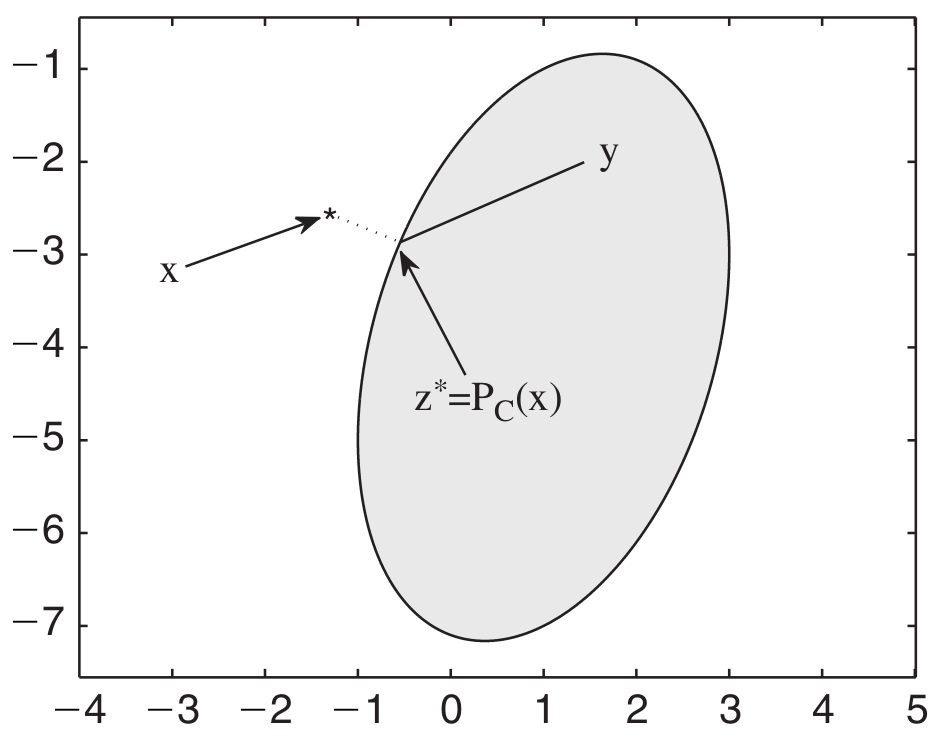
\includegraphics[width=0.5\linewidth]{second_projection}.
	\caption{The orthogonal projection operator.} \label{fig:second_projection}
\end{figure}
\begin{theorem}[Second Projection Theorem]\label{thm:second_projection}
	Let $C$ be a nonempty closed convex set. Then $z=P_C(x)$ iff 
	\begin{equation}\label{eq:second_projection}
		(x-z)^T(y-z) \leq 0\quad \forall \,y\in C.
	\end{equation}
\end{theorem}
\begin{proof}
	$z=P_C(x)$ iff it is the optimal solution of \eqref{eq:projection} iff (by Theorem \ref{thm:convex_stationarity})
	\begin{equation*}
		\grad(z)^T(y-z)\geq 0 \quad \forall\,y\in C,
	\end{equation*}
which concludes the proof as $\grad(z) = 2(x-z).$
\end{proof}
Another important property of the orthogonal projection operator is given in the
following theorem, which also establishes the so-called nonexpansiveness property of $P_C$.
\begin{theorem}[Nonexpansiveness of the projection operator]
	Let $C$ be a closed and convex set. Then, for any $v,w\in \Rn$
	\begin{itemize}
		\item[a)] 
		\begin{equation}\label{eq:nonexpansiveness_1}
			(P_C(v)-P_C(w))^T(v-w)\geq ||P_C(v)-P_C(w)||^2
		\end{equation}
		\item[b)]
		\begin{equation}\label{eq:nonexpansiveness_2}
			 ||P_C(v)-P_C(w)||\leq ||v-w||.
		\end{equation}
	\end{itemize}
\end{theorem}
\begin{proof}
	From Theorem \ref{thm:second_projection} we have that for any $x \in \Rn$ and $y\in C$
	\begin{equation*}
		(x-P_C(x))^T(y-P_C(x)) \leq 0.
	\end{equation*}
Replacing $x=v$ and $y=P_C(w)$ we have
\begin{equation*}
	(v-P_C(v))^T(P_C(w)-P_C(v)) \leq 0.
\end{equation*}
Replacing, instead, $x=w$ and $y=P_C(v)$
\begin{equation*}
	(w-P_C(w))^T(P_C(v)-P_C(w)) \leq 0.
\end{equation*}
Now, summing the two inequalities we get
\begin{equation*}
	(P_C(w)-P_C(v))^T(v-w+P_C(w)-P_C(v)) \leq 0,
\end{equation*}
and hence, 
\begin{equation*}
	(P_C(v)-P_C(w))^T(v-w) \geq ||P_C(w)-P_C(v)||^2.
\end{equation*}
To prove \eqref{eq:nonexpansiveness_2}, we note that if $P_C(v) = P_C(w)$, the inequality is trivial. Thus, we assume $P_C(v) \neq P_C(w)$. Then by Cauchy-Schwartz, we have 
\begin{equation*}
	(P_C(v)-P_C(w))^T(v-w) \leq ||P_C(v)-P_C(w)|| \cdot||v-w||,
\end{equation*}
which combined with \eqref{eq:nonexpansiveness_1} gives 
\begin{equation*}
	||P_C(v)-P_C(w)||^2 \leq ||P_C(v)-P_C(w)|| \cdot||v-w||,
\end{equation*}
which concludes the proof as $P_C(v) \neq P_C(w)$.
\end{proof}
Coming back to stationarity, let us provide the alternative characterization of a stationary point through the projection operator. Notice that this theorem holds also when $f$ is non-convex. 
\begin{theorem}\label{thm:stationarity_projection}
	Let $f\in C^1(C)$ with $C$ closed and convex and let $s>0$. $x^*$ is a stationary point of the problem \eqref{eq:problem} iff 
	\begin{equation}\label{eq:stationary_projection}
		x^*=P_C(x^*-s\grad(x^*)).
	\end{equation}
\end{theorem}
\begin{proof}
	By the second projection theorem (Theorem \ref{thm:second_projection}), we get that $x^*=P_C(x^*-s\grad(x^*))$ iff
	\begin{equation*}
		(x^*-s\grad(x^*) -x^*)^T(x-x^*)\leq 0, 
	\end{equation*}
which concludes the proof, as $x^*$ is a stationary point when $\grad(x^*)^T(x-x^*)\geq0$
\end{proof}
\subsection{Projected Gradient Descent}
The characterization of stationary points through equation \eqref{eq:stationary_projection} directly suggest a new algorithm for solving convex constrained optimization methods. As we will see later, this algorithm finds stationary points despite $f$ being convex or not. \\
\begin{algorithm}[H]\label{alg}
	\caption{Projected Gradient Descent (PGD)}
	
	\KwIn{$x_0\in \Rn$, $\epsilon>0$, $t\in (0,\frac{L}{2})$}
	
	$k = 0$
	
	\While{$||x_{k-1}-x_k||> \epsilon$}{
				
		$x_{k+1} = P_C(x_k-t\grad(x_k)$
		
		$k = k+1$
	}
\end{algorithm}
The proof of convergence of PGD is similar to that of GD. In particular, we first prove the Descent Lemma (part 2) for constrained optimization problem. Notice that the the Descent Lemma (part 1) holds for any $x, y \in \Rn$.
\begin{lemma}[Descent Lemma (part 2) for Convex Constrained Problems]\label{lemma:descent_projected_lemma}
	Let $f\in \LC(C)$, where $C$ is convex and closed. Then for any $x\in C$ and $t\in (0,\frac{2}{L})$ the following inequality holds
	\begin{equation*}
		f(x)-f(P_C(x-t\grad(x))) \geq t\left(1- \frac{Lt}{2}\right) \left\| \frac{1}{t}(x-P_C(x-t\grad(x))) \right\|^2.
	\end{equation*}
\end{lemma}
\begin{proof}
	Exercise.
\end{proof}
\noindent It is now convenient to define the gradient mapping as
\begin{equation}\label{eq:gradient}
	G_M(x) := M \left(x-P_C\left(x-\frac{1}{M}\grad(x)\right)\right) \quad\with M>0.
\end{equation}
Note that in the unconstrained case $G_M(x)=\grad(x)$ so the gradient mapping is an extension of the usual gradient operator. In addition, by Theorem \ref{thm:stationarity_projection}, $G_M(x) = 0$ iff $x$ is a stationary point of \eqref{eq:problem}. This means that we can look at $\|G_M(x)\|$ as an optimality measure. Moreover, the sufficient decrease stated above can be rewritten as 
\begin{equation*}
	f(x)-f(P_C(x-t\grad(x))) \geq t\left(1- \frac{Lt}{2}\right) \left\| G_{\frac{1}{t}} (x) \right\|^2.
\end{equation*}
This generalized sufficient decrease property allows us to prove similar results to those proven in the unconstrained case.
\begin{theorem}[Convergence of PGD method]
	Let $f\in \LC(C)$, with $C$ closed and convex. Let $\{x_k\}_k$ be a sequence generated by Algorithm \ref{alg} for solving \eqref{eq:problem}. Assume that $f$ is bounded below over $C$. Then we have the following
	\begin{itemize}
		\item[(a)] The sequence $\{f(x_k)\}_k$ is nonincreasing. In addition, for any $k\geq 0$, $f(x_{k+1}) < f(x_k)$ unless $x_k$ is a stationary point.
		\item[(b)] $G_{\frac{1}{t}}(x_k) \to 0$ as $k\to \infty$.
	\end{itemize}
\end{theorem}
\begin{proof}
	Exercise.
\end{proof}
\noindent Notice that the theorem above only ensures convergence to a stationary point, which in the non-convex case might not be a global minimum. Also, the iteration complexity of PGD is the same as that of GD, that is $\BigO(\epsilon^{-2})$. If we assume $f$ to be convex, we can instead ensure a faster rate of convergence, moreover, thanks to Theorem \ref{thm:convex_stationarity} all stationary points of \eqref{eq:problem} are global minima.
\begin{theorem}[Convergence of PGD method for convex problems]
	Let $f\in \LC(C)$ be convex, with $C$ closed and convex. Let $\{x_k\}_k$ be a sequence generated by Algorithm \ref{alg} for solving \eqref{eq:problem} with $t\in (0,\frac{1}{L})$. Assume that the set of optimal solutions $X^*$ is nonempty and that $f^*$ is the optimal value. Then we have the following
	\begin{itemize}
		\item[(a)] for any $k\geq0$ and $x^*\in X^*$
		\begin{equation*}
			2t(f(x_{k+1}) -f^*) \leq ||x_k-x^*||^2 - ||x_{k+1}-x^*||^2,
		\end{equation*}
		\item[(b)] for any $T\geq 0$:
		\begin{equation*}
			f(x_T)-f^*\leq \frac{||x_0-x^*||}{2tT}.
		\end{equation*}
	\end{itemize}
\end{theorem}
\begin{proof}
	By the second projection theorem \eqref{eq:second_projection} applied on the projected point $x_{k+1}$, we have that 
	\begin{equation*}
		\left(x_k -t\grad(x_k) -x_{k+1}\right)^T\left(x^*-x_{k+1}\right)\leq 0
	\end{equation*}
	if and only if
	\begin{equation*}
		\grad(x_k)^T\left(x_{k+1}-x^*\right)+ \frac{1}{t}\left(x_k -x_{k+1}\right)^T\left(x^*-x_{k+1}\right)\leq0
	\end{equation*}
	if and only if
	\begin{equation}\label{eq:from_g_to_pg}
		\grad(x_k)^T\left(x_{k+1}-x^*\right) \leq \frac{1}{t}(x_k-x_{k+1})^T\left(x_{k+1}-x^*\right).
	\end{equation}
	By the Descent Lemma (part 1) , we have 
	\begin{equation*}
		f(x_{k+1}) \leq f(x_k)+\grad(x_k)^T(x_{k+1}-x_k) +\frac{L}{2}||x_{k+1}-x_k||^2.
	\end{equation*}
Let $x^*$ be a global minimum of \eqref{eq:problem}, then the gradient characterization of convexity implies that $f(x_k)\leq f(x^*)+\grad(x_k)^T(x_k-x^*)$, which together with the previous inequality implies that
\begin{equation*}
	f(x_{k+1}) \leq f(x^*)+\grad(x_k)^T(x_k-x^*)+\grad(x_k)^T(x_{k+1}-x_k) +\frac{L}{2}||x_{k+1}-x_k||^2.
\end{equation*}
Thus, together with \eqref{eq:from_g_to_pg} and $t\leq \frac{1}{L}$, we get
\begin{equation*}
	\begin{split}
		f(x_{k+1}) &\leq f(x^*)+\grad(x_k)^T(x_k-x^*)+\grad(x_k)^T(x_{k+1}-x_k) +\frac{L}{2}||x_{k+1}-x_k||^2\\
		& = f(x^*)+\grad(x_k)^T(x_{k+1}-x^*) +\frac{L}{2}||x_{k+1}-x_k||^2\\
		&\leq f(x^*)+\frac{1}{t}(x_k-x_{k+1})^T\left(x_{k+1}-x^*\right)+\frac{L}{2}||x_{k+1}-x_k||^2\\
		&\leq f(x^*)+\frac{1}{t}(x_k-x_{k+1})^T\left(x_{k+1}-x^*\right)+\frac{1}{2t}||x_{k+1}-x_k||^2\\
		&= f(x^*)+\frac{1}{2t}(x_k-x_{k+1})^T\left(x_{k+1}-x^*+x_k - x^*\right)\\
		&= f(x^*)+\frac{1}{2t}(x_k-x_{k+1}+x^*-x^*)^T\left(x_{k+1}-x^*+x_k - x^*\right)\\
		&= f(x^*)+\frac{1}{2t}(x_k-x^*)^T\left(x_{k+1}-x^*+x_k - x^*\right) + \frac{1}{2t}(x^*-x_{k+1})^T\left(x_{k+1}-x^*+x_k - x^*\right)\\
		&= f(x^*)+\frac{1}{2t}\left(||x_k-x^*||^2+(x_k-x^*)^T(x_{k+1}-x^*)-(x_k-x^*)^T(x_{k+1}-x^*) -||x_{k+1}-x^*||^2\right)\\
		&= f(x^*)+\frac{1}{2t}\left(||x_k-x^*\|^2 -\|x_{k+1}-x^*\|^2\right)
	\end{split}
\end{equation*}
establishing part (a). To achieve (b), we sum the inequalities (a) for $k=0,1, \dots, T-1$ and obtain
\begin{equation*}
	||x_T-x^*\|^2 -\|x_0-x^*\|^2 \leq 2t \sum_{k=0}^{T-1} \left(f(x^*)-f(x_{k+1})\right) \leq 2tT(f(x^*)-f(x_T)),
\end{equation*}
where in the last inequality we used the fact that $f(x_{k+1})\leq f(x_k)$, which, in turn, is a consequence of the Descent Lemma (part 2) for convex constrained problems and the fact that $t\in(0, \frac{1}{L})$. Thus, 
\begin{equation*}
	f(x_T) -f(x^*) \leq \frac{||x_0-x^*\|^2 -\|x_T-x^*\|^2}{2tT}\leq \frac{||x_0-x^*\|^2}{2tT}.
\end{equation*}
\end{proof}

\noindent Notice that one crucial step in the proof is \eqref{eq:from_g_to_pg}, as this is what relates the gradient with the direction take after the projection.

\pagebreak


\section{Constrained Nonconvex Optimization}
In this chapter we will derive the necessary optimality conditions, i.e., Karush-Kunh-Tucker (KKT) conditions, for the most general case where the feasible set is possibly nonconvex. In particular, we consider problems of the following shape
\begin{equation}\label{eq:last_problem}
\begin{split}
\min \;\; &f(x)\\
\st& g_i(x)\leq 0, \quad i=0, \dots, m,
\end{split}
\end{equation}
where $f,g_i\in \C(\R)$ but possibly not convex. Notice that this class of problems is very general, as equality constraints can be included observing that $h(x)=0$ can be replaced by 2 inequalities $h(x)\leq0$ and $-h(x)\leq 0$. From now on $C:=\{x\in\Rn: g_i(x)\leq 0, \; i\in [m] \}$. 
\begin{definition}[Feasible Descent Direction] A vector $d$ is called feasible descent direction at $x\in C$ if $\grad(x)^Td<0$ and there exists $\epsilon>0$ such that $x+td\in C$ for all $t\in [0,\epsilon].$

\end{definition}
\noindent Obviously, a necessary local optimality condition of a point $x$ is that it does not have
any feasible descent directions.
\begin{lemma} Let $x^*$ be a local optimum of \eqref{eq:last_problem}, then there are no feasible descent directions at $x^*.$
\end{lemma}
\begin{proof}
The proof goes by contradiction and follows directly from the definition of feasible descent direction and directional derivative.
\end{proof}
\begin{definition}[Active Constraints] Let $g_i(x)\leq 0, \; i\in [m] $ be a set of inequalities. The active constraints at $x$ are the constraints satisfied as equalities at $x$. The set of active constraints is denoted by $I(x):=\{i\in[m]: g_i(x)=0\}.$
\end{definition}

\begin{lemma}\label{lemma:for_fritzjohn}
Let $x^*$ be a local minimum of the problem \eqref{eq:last_problem} and let $I(x^*)$ be the set of active constraints at $x^*$. Then, there does not exist a vector $d\in\Rn$ such that 
\begin{align*}
&\grad(x^*)^Td<0,\\
&\nabla g_i (x^*)^Td<0,\quad i \in I(x^*).
\end{align*}
\end{lemma}
\begin{proof}
Suppose by contradiction that $d$ satisfies the system of inequalities above. Then it follows that there exists $\epsilon_1>0$ such that $f(x^*+td)<f(x^*)$ and $g_i(x+td)<g(x^*)=0$ for any $t\in (0,\epsilon_1)$ and $i\in I(x^*)$. For any $i\not \in I(x^*)$, we have $g_i(x^*)<0$ and hence, by continuity of $g_i$ it follows that there exists $\epsilon_2>0$ such that $g_i(x^*+td)<0$ for any $t\in (0,\epsilon_2)$ and $i\not \in I$. We can thus conclude that 
\begin{align*}
&\grad(x^*+td)^Td<f(x^*),\\
&\nabla g_i (x^*+td)^Td<0,\quad i \in [m],
\end{align*}
for all $t\in (0,\min\{\epsilon_1,\epsilon_2\})$, which is a contradiction to the local optimality of $x^*$.
\end{proof}
We have thus shown that a necessary optimality condition for local optimality is the infeasibility of a certain system of strict inequalities. On the other hand, similarly to the stationarity condition, this system is difficult to use in practice. We will state now the Fritz-John conditions.
\begin{theorem}[Fritz-John Conditions]\label{thm:fritzjohn}
Let $x^*$ be a local minimum of the problem \eqref{eq:last_problem}. Then there exists multipliers $\lambda_0,\dots, \lambda_1, \dots, \lambda_m\geq0$ such that they are not all zeros and such that 
\begin{equation}\label{eq:fritzjohn}
\begin{split}
\lambda_0\grad(x^*)+ \sum_{i=1}^{m} \lambda_i \nabla g_i(x^*) &= 0,\\
\lambda_ig_i(x^*)&=0 \quad i=1, \dots, m.
\end{split}
\end{equation}
\end{theorem}
\begin{figure}
	\centering
	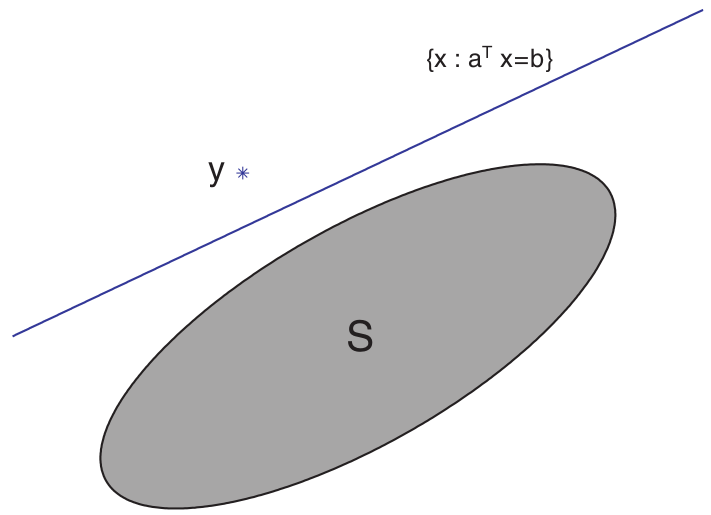
\includegraphics[width=0.5\linewidth]{separation}.
	\caption{Strict separation of point from a closed and convex set.} \label{fig:separtation}
\end{figure}
\noindent In order to prove this theorem we need a rather large digression into the Alternative Theorems. 
\subsection{Alternative Theorems}
We begin with a very simple yet powerful result on convex sets, namely the separation theorem between a point and a closed convex set. This result will be the basis for all the optimality conditions that will be discussed later on.
\begin{theorem}[Strict Separation Theorem]\label{thm:separation}
	Let $C$ be a closed and convex set and let $y\not \in C$. Then there exists $p\in \Rn \setminus \{0\}$ and $\alpha\in \R$ such that
	\begin{equation*}
		p^Ty>\alpha \qquad \text{and} \qquad p^Tx\leq \alpha \;\;\forall x\in C.
	\end{equation*}
\end{theorem}
\begin{proof}
By the second projection theorem, the vector $\bar{x}=P_C(y)\in C$ satisfies
\begin{equation*}
	(y-\bar{x})^T(x-\bar{x}) \leq 0 \;\; \forall x\in C
\end{equation*}
which is the same as 
\begin{equation*}
	(y-\bar{x})^T x \leq (y-\bar{x})^T \bar{x} \;\; \forall x\in C.
\end{equation*}
Denote $p=y-\bar{x}\neq 0$ (since $y\not \in C$) and $\alpha= (y-\bar{x})^T \bar{x}$. Then we have that $p^Tx\leq \alpha\;\forall x\in C$. On the other hand,
\begin{equation*}
	p^Ty = (y-\bar{x})^Ty = (y-\bar{x})^T(y-\bar{x}) + (y-\bar{x})^T\bar{x} = ||y-\bar{x}||^2 + \alpha > \alpha,
\end{equation*}
and the result is established.
\end{proof}
\noindent Now, before going on with two more alternative theorems, we need to show that the conic hull of a fine set is closed and convex.
\begin{definition}[Conic Hull] Let $S\subseteq \Rn$. Then the conic hull of $S$, denoted by $\cone(S)$,
	is the set comprising all the conic combinations of vectors from S:
	\begin{equation*}
		\cone(S):=\left\{\sum_{i=1}^k \lambda_i x_i: x_1,\dots, x_k\in S, \lambda\in \R^k_+, k \in \N\right\}
	\end{equation*}
\end{definition}
\begin{lemma}\label{lemma:cone}
	Let $a_1, a_2, \dots a_p\in \Rn$, $p\in \N$. Then $\cone(\{a_1, \dots, a_p\})$ is closed and convex.
\end{lemma}
\begin{proof}
	Exercise.
\end{proof}
\noindent We can now go on with the next alternative theorem.
\begin{lemma}[Farkas' lemma, second formulation]\label{lemma:farkas}
	Let $c\in \Rn$ and $A\in \Rmn.$ Then the following two claims are equivalent:
	\begin{itemize}
		\item[M.] The implication $Ax\leq 0 \Rightarrow c^Tx\leq 0$ holds true. 
		\item[N.] There exists $y\in \Rn_+$ such that $A^Ty=c.$
	\end{itemize}
\end{lemma}
\begin{proof}
	Suppose that system $N$ is feasible. To see that the implication $M$ holds, suppose that $Ax\leq 0$ for some $x\in \Rn$. Then, multiplying this inequality from the left by $y^T$ (a valid operation since $y\geq0$) yields 
	\begin{equation*}
		y^TAx\leq 0,
	\end{equation*}
which concludes the thesis by noticing that $c^T=y^TA$. 
\par The reverse direction is not so obvious. Suppose that the implication $M$ is satisfied, and
let us show that system $N$ is feasible. Suppose by contradiction that system $N$ is infeasible,
and consider the following set
\begin{equation*}
	S=\{x\in\Rn: x= A^Ty \; y\in \Rn_+\},
\end{equation*}
which is closed and convex thanks to Lemma \ref{lemma:cone}. The infeasibility of N means that $c\not \in S$, otherwise $c$ would be a solution of N. By Theorem \ref{thm:separation}, it follows that there exists a vector $p\in \Rn \setminus \{0\}$ and $\alpha\in \R$ such that $p^Tc>\alpha$ and 
\begin{equation}\label{eq:farkas_final}
	p^Tx\leq \alpha \; \forall x\in S
\end{equation}
Since $0\in S$, from \eqref{eq:farkas_final} we have that $\alpha\geq 0$ and hence also $p^Tc>0$. In addition, \eqref{eq:farkas_final} is equivalent to 
\begin{equation*}
	p^TA^Ty\leq \alpha \;\; \forall y\geq 0 
\end{equation*}
or to 
\begin{equation}\label{eq:contradicting_ineq}
	(Ap)^Ty\leq \alpha \;\; \forall y\geq 0.
\end{equation}
By showing that $Ap \leq 0$, we would find a vector $p$ for which $Ap\leq 0$ and $c^Tp>0$, which contradicts the implication $M$. Thus, let us now prove that $Ap \leq 0$ (notice that this means component-wise).  By contradiction, if there was an index $i\in \{1,2, \dots,m\}$ such that $(Ap)_i>0$, then for $y=\beta e_i$ we would have that $(Ap)^Ty = \beta (Ap)_i$ which is an expression that goes to $\infty$ as $\beta\to \infty$, and, thus, cannot be bounded by a constant $\alpha$ as proved for \eqref{eq:contradicting_ineq}.
\end{proof}
\noindent In order to prove Gordon's alternative theorem, we are going to use Farkas' lemma in the following formulation.
\begin{lemma}[Farkas' lemma, first formulation]\label{lemma:Farkas}
	Let $c\in \Rn$ and $A\in \Rmn.$ Then exactly one of the following system has a solution:
	\begin{itemize}
		\item[I.] $Ax\leq 0, c^Tx> 0$. 
		\item[II.] $A^Ty=c, y\geq 0$.
	\end{itemize}
\end{lemma}
\noindent To show that the two formulations are equivalent, let us notice that $II$ is equivalent to $N$ and let us write down the truth table of $M$ and $I$. In particular, let us call $M_1$ the statement $Ax\leq 0$ and $M_2$ the statement $c^Tx\leq0$ and notice that $I=M_1 \wedge \bar{M}_2$.\\

\begin{tabular}{|c|c|c|c|}
	\hline
	M$_1$& M$_2$ & M= M$_1\Rightarrow$M$_2$& $I=M_1 \wedge \bar{M}_2$ \\
	\hline
	F& F & T & F \\
	\hline
	F& T & T & F \\
	\hline
	T& F & F & T \\
	\hline
	T& T & T & F \\
	\hline
\end{tabular}\\[1\baselineskip]
In particular, this means that the two formulations are equivalent as the first formulation (Lemma \ref{lemma:Farkas}) states that exactly one between $I$ and $II$ has solutions while the second formulation (Lemma \ref{lemma:farkas}) states that $M$ and $N$ are equivalent.

\begin{theorem}[Gordon's Alternative Theorem]\label{thm:gordon}
	Let $A\in\Rmn$. Then exactly one of the following statements has a solution:
	\begin{itemize}
		\item[M.] $Ax<0$.
		\item[N.] $p\neq 0, A^Tp = 0, p\geq 0$.
	\end{itemize}
\end{theorem}
\begin{proof}
	Suppose that the system $M$ has a solution. We will prove that $N$ is infeasible. Assume by contradiction that $N$ is feasible, meaning that there exists $p\neq0$ satisfying $A^Tp=0, p\geq0$. Multiplying the equality $A^Tp=0$ from the left by $x^T$ yields 
	\begin{equation*}
		(Ax)^Tp=0
	\end{equation*}
which is impossible since $Ax<0$ and $0\neq p\geq0$.
\par Now suppose that the system $M$ does not have a solution. Note that the system $M$ is equivalent to 
\begin{align*}
	Ax+se&\leq 0\\
	s&>0, s\in \R. 
\end{align*}
The latter system can be rewritten as 
\begin{equation*}
	\tilde{A}\begin{pmatrix}
		x\\
		s
	\end{pmatrix}\leq 0, \qquad c^T\begin{pmatrix}
	x\\
	s
\end{pmatrix}>0,
\end{equation*}
where $\tilde{A}=(A e)$ and $c=e_{n+1}$. The infeasibility of $M$ is thus equivalent to the infeasibility of the system 
\begin{equation*}
\tilde{A}w\leq 0, \quad c^Tw>0,\quad w\in \R^{n+1}.
\end{equation*}
By Farkas' lemma, there exists $z\in \R^{m}_+$ such that 
\begin{equation*}
	\begin{pmatrix}
		A^T\\
		e^T
	\end{pmatrix}z = c,
\end{equation*}
that is, there exists $z\in \R^m_+$ such that 
\begin{equation*}
	A^Tz=0, \qquad e^Tz=1.
\end{equation*}
Since $ e^Tz=1$ it follows in particular that $z\neq 0$, and we have thus shown the existence of $0\neq z \in \R^m_+$ such that $A^Tz=0$, that is $N$ is feasible.
\end{proof}

\subsection{KKT Conditions}
Before stating and proving the KKT conditions, we first prove Theorem \ref{thm:fritzjohn}.
\begin{proof}[Proof of Theorem \ref{thm:fritzjohn}]
	By Lemma \ref{lemma:for_fritzjohn} it follows that the following system of inequality does not have a solution:
	\begin{equation}\label{eq:system_for_fritzjohn}
		\begin{split}
			\grad(x^*)^Td<0,\\
			\nabla g_i(x^*)^Td<0 \quad i\in I(x^*),
		\end{split}
	\end{equation}
where $I(x^*)=\{i_1, i_2, \dots, i_k\}$. System \eqref{eq:system_for_fritzjohn} can be rewritten as 
\begin{equation*}
	Ad<0,
\end{equation*}
where 
\begin{equation*}
	A=\begin{pmatrix}
		\grad(x^*)^T\\
		\nabla g_{i_1}(x^*)^T\\
		\vdots\\
		\nabla g_{i_k}(x^*)^T
	\end{pmatrix}
\end{equation*}
By Gordon's theorem of the alternative (Theorem \ref{thm:gordon}), system \eqref{eq:system_for_fritzjohn} is infeasible iff there exists a vector $\eta=(\lambda_0, \lambda_{i_1}, \dots, \lambda_{i_k})^T\neq 0$ such that 
\begin{equation*}
	A^T\eta = 0, \qquad \eta\geq 0,
\end{equation*}
which is the same as 
\begin{equation*}
	\begin{split}
		\lambda_0 \grad(x^*) + \sum_{i\in I(x^*)} \lambda_i \nabla g_i(x^*) &= 0,\\
		\lambda_i&\geq 0, \quad i \in I(x^*).
	\end{split}
\end{equation*}
Define $\lambda_i=0$ for any $i\not \in I(x^*)$, and we obtain that 
\begin{equation*}
	\lambda_0 \grad(x^*) + \sum_{i=1}^{m} \lambda_i\nabla g_i(x^*)=0
\end{equation*}
and that $\lambda_i g_i(x^*)=0$ for any $i\in [m]$ as required.
\end{proof}
A major drawback of the Fritz-John conditions is in the fact that they allow $\lambda_0$ to be
zero. This case is not particularly informative as when $\lambda_0=0$ the Fritz-John conditions simply means that the gradients of the active constraints are linearly dependent. This condition has nothing to do with the objective function, implying that
there might be a lot of points satisfying the Fritz-John conditions which are not local minimum points. If we add an assumption that the gradients of the active constraints are linearly independent at $x^*$, then we can establish the KKT conditions, which are the same as the Fritz-John conditions with $\lambda_0 = 1$. Before introducing them, let us define the Lagrangian of problem \eqref{eq:last_problem}
\begin{equation}\label{eq:lagrange}
	L(x,\lambda) = f(x) +\sum_{i=1}^m \lambda_i g_i(x),
\end{equation}
where $\lambda_1, \dots, \lambda_m$ are the nonnegative Lagrange multipliers associated to the inequalities $g_1, \dots, g_m$.

\begin{theorem}[KKT conditions]
	Let $x^*$ be a local minimum of the problem \eqref{eq:last_problem}, with $f, g_1,\dots, g_m\in \C(\Rn)$. Let $I(x^*)$ be the set of active constraints and suppose that the gradients of the active constraints $\{\nabla g_i(x^*)\}_{i\in I(x^*)}$ are linearly independent. Then there exists multipliers $\lambda_1, \dots, \lambda_m\geq 0$ such that 
	\begin{equation}\label{eq:kkt}
		\begin{split}
			\nabla_x L(x^*,\lambda) = \grad(x^*)+ \sum_{i=1}^{m} \lambda_i \nabla g_i(x^*) &= 0,\\
			\lambda_ig_i(x^*)&=0 \quad i=1, \dots, m.
		\end{split}
	\end{equation}
\end{theorem}
\begin{proof}
	By Fritz-John it follows that there exist $\tilde{\lambda}_0, \tilde{\lambda}_1, \dots, \tilde{\lambda}_m\geq 0$ not all zeros, such that \begin{equation*}
		\begin{split}
			\tilde{\lambda}_0\grad(x^*)+ \sum_{i=1}^{m} \tilde{\lambda}_i \nabla g_i(x^*) &= 0,\\
			\tilde{\lambda}_ig_i(x^*)&=0 \quad i=1, \dots, m.
		\end{split}
	\end{equation*}
In particular, $\tilde{\lambda}_0\neq0$ otherwise the gradients of the active constraints would be linearly dependent, against the assumption of being linearly independent. The KKT-multipliers are simply defined as $\lambda_i=\frac{\tilde{\lambda}_i}{\lambda_0}$.
\end{proof}
\begin{remark}[Constraint Qualifications]
	The condition that the gradients of the active constraints are linearly independent
	is one of many types of assumptions that are referred to in the literature as ``constraint
	qualifications.'' These are the conditions on the constraints that imply the KKT points to be necessary conditions for optimality. The points satisfying these conditions are usually called ``regular''. Famous constraint qualifications are 
	\begin{itemize}
		\item Linear Independence Constraint Qualification (LICQ), the ones just mentioned.
		\item Linear CQ (LCQ), $g_i$ are affine functions.
		\item Mangasarian-Fromovitz CQ (MFCQ) \cite{mangasarian67a}. MFCQ holds at a feasible point $x^*$ if there exists a vector $d \in \mathbb{R}^n$ such that:
		$$\nabla g_j(x^*)^T d < 0, \quad \forall j \in I(x^*)$$
		\item Constant Positive Linear Dependence Constraint Qualification (CPLD): CPLD holds at $x^*$ if for every finite subset $S \subseteq I(x^*)$ and every collection of positive scalars $\{\lambda_j\}_{j \in S}$ with $\lambda_j > 0$ such that
		$$\sum_{j \in S} \lambda_j \nabla g_j(x^*) = 0$$
		there exists a neighborhood $U$ of $x^*$ such that for all $x \in U$:
		$$\sum_{j \in S} \lambda_j \nabla g_j(x) = 0$$
		\item Slater's conditions: $f$ and $g_i$ are convex and the feasible set is non-empty.
	\end{itemize}
	LICQ$\Rightarrow$MFCQ$\Rightarrow$CPLD$\Rightarrow$Quasi-Normality CG (QNCQ)
\end{remark}
\begin{remark}[Drawbacks of the KKT conditions]
	$ $
	\begin{itemize}
\item By construction, solving (exactly) the KKT conditions will only allow you to find KKT points which are regular, but there might be better non-regular points. Take the extreme case of the problem $\min x\; \; s.t. x^2=0$, where the set of KKT points is empty but the solution exists and it is $x^*=0$.
\item Solving the KKT system \eqref{eq:kkt} does not ensure the feasibility of $x$. One needs to take into account also the constraints of \eqref{eq:last_problem}. In fact, notice that the KKT are ``only'' necessary conditions for a feasible local minimum.
\end{itemize}
\end{remark}
\noindent Rewriting \eqref{eq:kkt} as 
\begin{equation}\label{eq:final_system}
	B (x,\lambda) :=
	\begin{pmatrix}
		\grad(x)+ \sum_{i=1}^{m} \lambda_i \nabla g_i(x)\\
		\lambda_1 g_1(x)\\
		\vdots\\
		\lambda_m g_m(x)\\
	\end{pmatrix}=0,
\end{equation}
one could solve the second issue above by using some new variables $w$ to ensure that the constraints are satisfied, i.e., $g_i(x)+w_i=0$ with $w\in \R^m_+$ is equivalent to $g_i(x)\leq 0$. This variables are called ``slack'' variables as they would relax the constraints if one does not enforce them to be non-negative. Also, $w_i=0$ if and only if the corresponding constraint $g_i$ is active. Thus, the system \eqref{eq:final_system} equipped with the constraints $g_i\leq 0$ is equivalent to 
\begin{equation*}
	A (x,\lambda,w) :=
	\begin{pmatrix}
		\grad(x)+ \sum_{i=1}^{m} \lambda_i \nabla g_i(x)\\
		\lambda_1 w_1\\
		\vdots\\
		\lambda_m w_m\\
		g_1(x) + w_1\\
		\vdots\\
		g_m(x) +w_m\\
	\end{pmatrix}=0.
\end{equation*}
Notice that $A:\Rn\times\R^m_+\times\R^m_+\to \R^{2m+1}$ is generally nonlinear and non-convex. Now, we can define the merit function of this system as $F(x,\lambda,w) := \frac{1}{2}||A(x,\lambda,w)||^2$ and solve instead the following optimization problem
\begin{equation*}
	\begin{split}
		\min \;\; &F(x,\lambda, w)= \frac{1}{2}||A(x,\lambda,w)||^2\\
		\st& \lambda\geq 0\\
		& w\geq 0.
	\end{split}
\end{equation*}
Note that the above problem has convex constraints for which a projection is extremely easy (box-constraints), thus solving this problem with projected gradient will both aim at constructing solutions that are feasible and optimal. On the other hand, $F$ might not be convex, so the problem may not be solved to a global optimum ($A(x,\lambda,w)=0$). In this case, the solution $x^*$ may not be feasible and it may be need to be projected onto the feasible set. One could also consider solving the original problem ignoring the constraints and projecting the solution back to the feasible set only at the end. However, this approach is not always possible (e.g., consider a system that can only be evaluated within certain parameters) and may result in solutions that are arbitrary far from the feasible set. The KKT system instead automatically encapsulates the idea that one should move into the direction of the gradient as long as it is far from an active constraint.
\section{Duality}
Consider the general model
\begin{equation}\label{eq:primal}
	\begin{aligned}
		f^* &= \min \quad f(x) \\
		&\text{s.t.} \quad g_i(x) \leq 0, \quad i = 1, 2, \ldots, m, \\
		&\phantom{\text{s.t.}} \quad h_j(x) = 0, \quad j = 1, 2, \ldots, p, \\
		&\phantom{\text{s.t.}} \quad x \in X,
	\end{aligned}
\end{equation}
where $f$, $g_i$, $h_j$ ($i = 1, 2, \ldots, m$, $j = 1, 2, \ldots, p$) are functions defined on the set $X \subseteq \mathbb{R}^n$.
Problem \eqref{eq:primal} will be referred to as the primal problem. At this point, we do not assume
anything on the functions (they are not even assumed to be continuous). The Lagrangian
of the problem is
\begin{equation*}
	L(x, \lambda, \mu) = f(x) + \sum_{i=1}^{m} \lambda_i g_i(x) + \sum_{j=1}^{p} \mu_j h_j(x) \quad (x \in X, \lambda \in \mathbb{R}_+^m, \mu \in \mathbb{R}^p),
\end{equation*}
where $\lambda_1, \lambda_2, \ldots, \lambda_m$ are nonnegative Lagrange multipliers associated with the inequality constraints, and $\mu_1, \mu_2, \ldots, \mu_p$ are the Lagrange multipliers associated with the equality constraints. The dual objective function $q : \mathbb{R}_+^m \times \mathbb{R}^p \to \mathbb{R} \cup \{-\infty\}$ is defined to be
\begin{equation}\label{eq:dual_objective}
	q(\lambda, \mu) = \min_{x \in X} L(x, \lambda, \mu).
\end{equation}
Note that we use the ``min'' notation even though the minimum is not necessarily attained.
In addition, the optimal value of the primal problem in \eqref{eq:dual_objective} is not always finite, there are values of $(\lambda, \mu)$ for which $q(\lambda, \mu) = -\infty$.\\
$-q(\lambda, \mu)$ is an \textbf{extended real-valued function}, i.e., a function that takes values in $\R \cup \{\infty\}$. The \textbf{effective domain} of an extended real-valued function is the set of vectors for which the function takes a finite value, so the domain of $q$ is 
\begin{equation*}
	\text{dom}(q) = \{(\lambda, \mu) \in \mathbb{R}_+^m \times \mathbb{R}^p : q(\lambda, \mu) > -\infty\}.
\end{equation*}
A generic extended real-valued function $f : \mathbb{R}^n \to \mathbb{R} \cup \{\infty\}$ is called \emph{proper} if it is not always equal to $\infty$, meaning that its effective domain is not empty. Similarly to the definition for finite-valued functions, an extended real-valued function is convex if for any $\mathbf{x}, \mathbf{y} \in \mathbb{R}^n$ and $\lambda \in [0,1]$ the following inequality holds:
\begin{equation*}
	f(\lambda \mathbf{x} + (1-\lambda)\mathbf{y}) \leq \lambda f(\mathbf{x}) + (1-\lambda)f(\mathbf{y}),
\end{equation*}
where we use the usual arithmetic with $\infty$:
\begin{equation*}
	a + \infty = \infty \text{ for any } a \in \mathbb{R},
\end{equation*}
\begin{equation*}
	a \cdot \infty = \infty \text{ for any } a \in \mathbb{R}_{++}.
\end{equation*}
In addition, we have the much less obvious rule that $0 \cdot \infty = 0$. 

For general extended real value function, an important set associated with them is their \textbf{epigraph}. Suppose that $f : \mathbb{R}^n \to \mathbb{R} \cup \{\infty\}$. Then the epigraph set $\text{epi}(f) \subseteq \mathbb{R}^{n+1}$ is defined by
\begin{equation*}
	\text{epi}(f) = \left\{ \begin{pmatrix} \mathbf{x} \\ t \end{pmatrix} : f(\mathbf{x}) \leq t \right\}.
\end{equation*}
\noindent An example of an epigraph can be seen in Figure \ref{fig:epigrph}. It is not difficult to show that an extended real-valued (or a real-valued) function $f$ is convex if and only if its epigraph set $\text{epi}(f)$ is convex (Exercise). 

\begin{figure}[h]
	\centering
	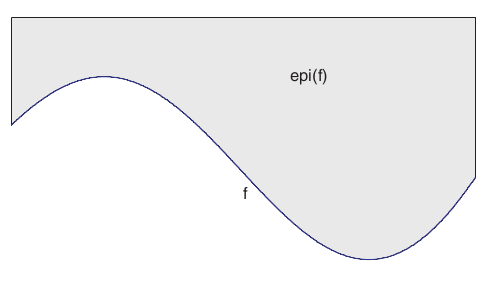
\includegraphics[width=0.5\linewidth]{epigraph}
	\caption{The epigraph of a one-dimensional function.}
	\label{fig:epigrph}
\end{figure}
\noindent An important property of convex extended real-valued functions that convexity is preserved under the maximum operation. 
\begin{theorem}[Preservation of Convexity under Maximum]\label{thm:max_is_convex}
	Let $f_i : \mathbb{R}^n \to \mathbb{R} \cup \{\infty\}$ be an extended real-valued convex function for any $i \in I$ ($I$ being an arbitrary index set). Then the function $f(\mathbf{x}) = \max_{i \in I} f_i(\mathbf{x})$ is an extended real-valued convex function.
\end{theorem}
\begin{proof}
	The result follows from the fact that $\text{epi}(f) = \bigcap_{i \in I} \text{epi}(f_i)$. The convexity of $f_i$ for any $i \in I$ implies the convexity of $\text{epi}(f_i)$ for any $i \in I$. Consequently, $\text{epi}(f)$, as an intersection of convex sets, is convex, and hence the convexity of $f$ is established. 
\end{proof}

\noindent Now, coming back to $q$, we can use this function to define the dual problem of \eqref{eq:primal}
\begin{equation}\label{eq:dual}
	\begin{aligned}
		q^* &= \max \quad q(\lambda, \mu) \\
		&\text{s.t.} \quad (\lambda, \mu) \in \text{dom}(q).
	\end{aligned}
\end{equation}

\noindent We begin by showing that the dual problem is always convex; it consists of maximizing a
concave function over a convex feasible set.

\begin{theorem}[Convexity of the Dual Problem]
	Consider problem \eqref{eq:primal} with $f$, $g_i$, $h_j$
	($i = 1, 2, \ldots, m$, $j = 1, 2, \ldots, p$) being finite valued functions defined on the set $X \subseteq \mathbb{R}^n$, and
	let $q$ be the function defined in \eqref{eq:dual_objective}. Then
	\begin{itemize}
		\item[(a)] dom$(q)$ is a convex set,
		\item[(b)] $q$ is a concave function over dom$(q)$.
	\end{itemize}
\end{theorem}

\begin{proof}
	
(a) To establish the convexity of dom$(q)$, take $(\lambda_1, \mu_1), (\lambda_2, \mu_2) \in$ dom$(q)$ and $\alpha \in
[0, 1]$. Then by the definition of dom$(q)$ we have that
\begin{equation*}
	\min_{x \in X} L(x, \lambda_1, \mu_1) > -\infty,
\end{equation*}
\begin{equation*}
	\min_{x \in X} L(x, \lambda_2, \mu_2) > -\infty.
\end{equation*}
Therefore, since the Lagrangian $L(x, \lambda, \mu)$ is affine with respect to $\lambda, \mu$, we obtain that
\begin{align*}
	q(\alpha \lambda_1 + (1-\alpha) \lambda_2, \alpha \mu_1 + (1-\alpha) \mu_2) &= \min_{x \in X} L(x, \alpha \lambda_1 + (1-\alpha) \lambda_2, \alpha \mu_1 + (1-\alpha) \mu_2) \\
	&= \min_{x \in X} \left[ \alpha L(x, \lambda_1, \mu_1) + (1-\alpha) L(x, \lambda_2, \mu_2) \right] \\
	&\geq \min_{x \in X} \left[ \alpha L(x, \lambda_1, \mu_1)\right] +  \min_{x \in X}   \left[(1-\alpha) L(x, \lambda_2, \mu_2) \right]\\
	&= \alpha \min_{x \in X} L(x, \lambda_1, \mu_1) + (1-\alpha) \min_{x \in X} L(x, \lambda_2, \mu_2) \\
	&= \alpha q(\lambda_1, \mu_1) + (1-\alpha) q(\lambda_2, \mu_2) \\
	&> -\infty,
\end{align*}
where the first inequality follows from the fact that if $x^*$ is the minimizer of the sum of $f(x)$ and $g(x)$, then $f(x^*)\geq \min_x f(x)$ and the same for $g$.  
Hence, $\alpha(\lambda_1, \mu_1) + (1-\alpha)(\lambda_2, \mu_2) \in$ dom$(q)$, and the convexity of dom$(q)$ is established.

(b) As noted in the proof of part (a), $L(x, \lambda, \mu)$ is an affine function with respect to
$(\lambda, \mu)$. It is in particular a concave function with respect to $(\lambda, \mu)$. Hence, since $q(\lambda, \mu)$ is
the minimum of concave functions (we minimize over all $x$, for each $x$ there is a concave function $L(x,\cdot)$) it must be concave. This follows immediately from
the fact that the maximum of convex functions is a convex function (Theorem \ref{thm:max_is_convex}). 
\end{proof} 

%Note that $-q$ is in fact an extended real-valued convex function over $\mathbb{R}_+^m \times \mathbb{R}^p$ as defined in Section 7.7, and the effective domain of $-q$ is exactly the domain defined in this section.
\noindent The first important result is closely connected to the motivation of the construction of the dual problem: the optimal dual value is a lower bound on the optimal primal
value. This result is called the weak duality theorem, and unsurprisingly, its proof is rather
simple.

\begin{theorem}[Weak Duality Theorem]\label{thm:weak_duality}
	Consider the primal problem \eqref{eq:primal} and its dual problem \eqref{eq:dual}. Then
	\begin{equation*}
		q^* \leq f^*,
	\end{equation*}
	where $q^*$, $f^*$ are the optimal dual and primal values respectively.
\end{theorem}

\begin{proof}
	Let us denote the feasible set of the primal problem by
	\begin{equation*}
		S = \{x \in X : g_i(x) \leq 0, h_j(x) = 0, i = 1, 2, \ldots, m, j = 1, 2, \ldots, p\}.
	\end{equation*}
	Then for any $(\lambda, \mu) \in \mathbb{R}_+^m \times \mathbb{R}^p$ we have
	\begin{align*}
		q(\lambda, \mu) &= \min_{x \in X} L(x, \lambda, \mu) \\
		&\leq \min_{x \in S} L(x, \lambda, \mu) \\
		&= \min_{x \in S} \left[ f(x) + \sum_{i=1}^{m} \lambda_i g_i(x) + \sum_{j=1}^{p} \mu_j h_j(x) \right] \\
		&\leq \min_{x \in S} f(x),
	\end{align*}
	where the last inequality follows from the fact that $\lambda_i \geq 0$ and for any $x \in S$, $g_i(x) \leq
	0, h_j(x) = 0$ ($i = 1, 2, \ldots, m, j = 1, 2, \ldots, p$). We thus obtain that
	\begin{equation*}
		q(\lambda, \mu) \leq \min_{x \in S} f(x)
	\end{equation*}
	for any $(\lambda, \mu) \in \mathbb{R}_+^m \times \mathbb{R}^p$. By taking the maximum over $(\lambda, \mu) \in \mathbb{R}_+^m \times \mathbb{R}^p$, the result
	follows.
\end{proof}

\subsection{Strong Duality in the Convex Case}

In the convex case we can prove under rather mild conditions that strong duality holds;
that is, the primal and dual optimal values coincide. Similarly to the derivation of the
KKT conditions, we will rely on separation theorems in order to establish the result.
The strict separation theorem (Theorem \ref{thm:separation}) states that a point can
be strictly separated from any closed and convex set. We will require a variation of this
result stating that a point can be separated from any convex set, not necessarily closed.
Note that the separation is not strict, and in fact it also includes the case in which the
point is on the boundary of the convex set and the theorem is hence called the \emph{supporting
	hyperplane theorem}.

\begin{theorem}[Supporting Hyperplane Theorem]\label{thm:supporting_hyperplane}
	Let $C \subseteq \mathbb{R}^n$ be a convex set and let $\mathbf{y} \notin C$. Then there exists $\mathbf{0} \neq \mathbf{p} \in \mathbb{R}^n$ such that
	\begin{equation*}
		\mathbf{p}^T \mathbf{x} \leq \mathbf{p}^T \mathbf{y} \text{ for any } \mathbf{x} \in C.
	\end{equation*}
\end{theorem}

\begin{proof}
	Since $\mathbf{y} \notin \text{int}(C)$, it follows that $\mathbf{y} \notin \text{int}(\text{cl}(C))$ (int$(C) = $ int$(\text{cl}(C))$, Exercise). Therefore, there exists a sequence $\{\mathbf{y}_k\}_{k \geq 1}$ satisfying $\mathbf{y}_k \notin \text{cl}(C)$
	such that $\mathbf{y}_k \to \mathbf{y}$. Since $\text{cl}(C)$ is convex (Exercise) and closed by its definition,
	it follows by the strict separation theorem (Theorem \ref{thm:separation}) that there exists $\mathbf{0} \neq \mathbf{p}_k \in \mathbb{R}^n$
	such that
	\begin{equation*}
		\mathbf{p}_k^T \mathbf{x} < \mathbf{p}_k^T \mathbf{y}_k
	\end{equation*}
	for all $\mathbf{x} \in \text{cl}(C)$. Dividing the latter inequality by $\|\mathbf{p}_k\| \neq 0$, we obtain
	\begin{equation}\label{eq:supporting_hyperplane}
		\frac{\mathbf{p}_k^T}{\|\mathbf{p}_k\|}(\mathbf{x} - \mathbf{y}_k) < 0 \text{ for any } \mathbf{x} \in \text{cl}(C).
	\end{equation}
	Since the sequence $\left\{ \frac{\mathbf{p}_k}{\|\mathbf{p}_k\|} \right\}_{k \geq 1}$ is bounded, it follows that there exists a subsequence $\left\{ \frac{\mathbf{p}_{k_\ell}}{\|\mathbf{p}_{k_\ell}\|} \right\}_{\ell \geq 1}$
	such that $\frac{\mathbf{p}_{k_\ell}}{\|\mathbf{p}_{k_\ell}\|} \to \mathbf{p}$ as $k \to \infty$ for some $\mathbf{p} \in \mathbb{R}^n$. Obviously, $\|\mathbf{p}\| = 1$ and hence in particular $\mathbf{p} \neq \mathbf{0}$. Taking the limit as $k \to \infty$ in inequality \eqref{eq:supporting_hyperplane}, we obtain that
	\begin{equation*}
		\mathbf{p}^T(\mathbf{x} - \mathbf{y}) \leq 0 \text{ for any } \mathbf{x} \in \text{cl}(C),
	\end{equation*}
	which readily implies the result since $C \subseteq \text{cl}(C)$.
\end{proof}


\begin{theorem}[Separation of Two Convex Sets]\label{thm:separation_sets}
	Let $C_1, C_2 \subseteq \mathbb{R}^n$ be two nonempty convex sets such that $C_1 \cap C_2 = \emptyset$. Then there exists $\mathbf{0} \neq \mathbf{p} \in \mathbb{R}^n$ for which
	\begin{equation*}
		\mathbf{p}^T \mathbf{x} \leq \mathbf{p}^T \mathbf{y} \text{ for any } \mathbf{x} \in C_1, \mathbf{y} \in C_2.
	\end{equation*}
\end{theorem}

\begin{proof}
	The set $C_1 - C_2:=\{x-y, x\in C_1, y\in C_2\}$ is a convex set (Exercise), and since $C_1 \cap C_2 = \emptyset$,
	it follows that $\mathbf{0} \notin C_1 - C_2$. By the supporting hyperplane theorem (Theorem \ref{thm:supporting_hyperplane}), it
	follows that there exists $\mathbf{0} \neq \mathbf{p} \in \mathbb{R}^n$ such that
	\begin{equation*}
		\mathbf{p}^T(\mathbf{x} - \mathbf{y}) \leq \mathbf{p}^T \mathbf{0} = 0 \text{ for any } \mathbf{x} \in C_1, \mathbf{y} \in C_2,
	\end{equation*}
	which is the same as the desired result.
\end{proof}

\noindent We will now derive a result which is a nonlinear version of Farkas lemma. The main difference is that a Slater-type condition must be assumed. Later on, this lemma will be
the key in proving the strong duality result.

\begin{theorem}[Nonlinear Farkas Lemma]\label{thm:nonlinear_farkas}
	Let $X \subseteq \mathbb{R}^n$ be a convex set and let $f, g_1, g_2, \ldots, g_m$ be convex functions over $X$. Assume that there exists $\hat{\mathbf{x}} \in X$ such that
	\begin{equation*}
		g_1(\hat{\mathbf{x}}) < 0, \quad g_2(\hat{\mathbf{x}}) < 0, \ldots, g_m(\hat{\mathbf{x}}) < 0.
	\end{equation*}
	Let $c \in \mathbb{R}$. Then the following two claims are equivalent.
	
	(a) The following implication holds:
	\begin{equation*}
		\mathbf{x} \in X, \quad g_i(\mathbf{x}) \leq 0, \quad i = 1, 2, \ldots, m \Rightarrow f(\mathbf{x}) \geq c.
	\end{equation*}
	
	(b) There exist $\lambda_1, \lambda_2, \ldots, \lambda_m \geq 0$ such that
	\begin{equation}\label{eq:farkas_b}
		\min_{\mathbf{x} \in X} \left\{ f(\mathbf{x}) + \sum_{i=1}^{m} \lambda_i g_i(\mathbf{x}) \right\} \geq c.
	\end{equation}
\end{theorem}

\begin{proof}
	The implication (b) $\Rightarrow$ (a) is rather straightforward. Indeed, suppose that there exist
	$\lambda_1, \lambda_2, \ldots, \lambda_m \geq 0$ such that \eqref{eq:farkas_b} holds, and let $\mathbf{x} \in X$ satisfy $g_i(\mathbf{x}) \leq 0, i = 1, 2, \ldots, m$.
	Then by \eqref{eq:farkas_b} we have that
	\begin{equation*}
		f(\mathbf{x}) + \sum_{i=1}^{m} \lambda_i g_i(\mathbf{x}) \geq c,
	\end{equation*}
	and hence, since $g_i(\mathbf{x}) \leq 0, \lambda_i \geq 0$,
	\begin{equation*}
		f(\mathbf{x}) \geq c - \sum_{i=1}^{m} \lambda_i g_i(\mathbf{x}) \geq c.
	\end{equation*}
	\noindent To prove that (a) $\Rightarrow$ (b), let us assume that the implication (a) holds. Consider the following two sets:
	\begin{align*}
		S &= \{u = (u_0, u_1, \ldots, u_m)\in \R^{m+1} : \exists \mathbf{x} \in X \text{ s.t. } f(\mathbf{x}) \leq u_0, g_i(\mathbf{x}) \leq u_i, i = 1, 2, \ldots, m\}, \\
		T &= \{u=(u_0, u_1, \ldots, u_m) \in \R^{m+1} : u_0 < c, u_1\leq 0, u_2 \leq 0, \ldots, u_m \leq 0\}.
	\end{align*}
Note that $S, T$ are nonempty and convex and in addition, by the validity of implication
(a), $S \cap T = \emptyset$. Therefore, by Theorem \ref{thm:separation_sets} (separation of two convex sets), it follows
that there exists a vector $\mathbf{a} = (a_0, a_1, \ldots, a_m) \neq \mathbf{0}$, such that
\begin{equation}\label{eq:separation_in_farkas}
	\min_{(u_0, u_1, \ldots, u_m) \in S} \sum_{j=0}^{m} a_j u_j \geq \max_{(u_0, u_1, \ldots, u_m) \in T} \sum_{j=0}^{m} a_j u_j.
\end{equation}
First note that $\mathbf{a} \geq \mathbf{0}$. This is due to the fact that if there was a negative component, say $a_j < 0$, then by taking $u_j$ to be a negative number tending to $-\infty$ while fixing all the other
components as zeros, we obtain that the right-hand-side maximum in \eqref{eq:separation_in_farkas} is $\infty$, which
is impossible. Since $\mathbf{a} \geq \mathbf{0}$, it follows that the right-hand side is $a_0 c$, and we thus obtain
\begin{equation}\label{eq:separation_reworked_in_farkas}
	\min_{(u_0, u_1, \ldots, u_m) \in S} \sum_{j=0}^{m} a_j u_j \geq a_0 c.
\end{equation}
Now we will show that $a_0 > 0$. Suppose in contradiction that $a_0 = 0$. Then
\begin{equation*}
	\min_{(u_0, u_1, \ldots, u_m) \in S} \sum_{j=1}^{m} a_j u_j \geq 0.
\end{equation*}
However, since we can take $u_i = g_i(\hat{\mathbf{x}}), i = 1, 2, \ldots, m$, we can deduce that
\begin{equation*}
	\sum_{j=1}^{m} a_j g_j(\hat{\mathbf{x}}) \geq 0,
\end{equation*}
which is impossible since $g_j(\hat{\mathbf{x}}) < 0$ for all $j$, and there exists at least one nonzero component in $(a_1, a_2, \ldots, a_m)$. Since $a_0 > 0$, we can divide \eqref{eq:separation_reworked_in_farkas} by $a_0$ to obtain
\begin{equation}\label{eq:in_farkas}
	\min_{(u_0, u_1, \ldots, u_m) \in S} \left\{ u_0 + \sum_{j=1}^{m} \tilde{a}_j u_j \right\} \geq c,
\end{equation}
where $\tilde{a}_j = \frac{a_j}{a_0}$. Define
\begin{equation*}
	\tilde{S} = \{u = (u_0, u_1, \ldots, u_m) : \exists \mathbf{x} \in X \text{ s.t. } f(\mathbf{x}) = u_0, g_i(\mathbf{x}) = u_i, i = 1, 2, \ldots, m\}.
\end{equation*}
Then obviously $\tilde{S} \subseteq S$. Therefore,
\begin{align*}
	\min_{(u_0, u_1, \ldots, u_m) \in S} \left\{ u_0 + \sum_{j=1}^{m} \tilde{a}_j u_j \right\} &\leq \min_{(u_0, u_1, \ldots, u_m) \in \tilde{S}} \left\{ u_0 + \sum_{j=1}^{m} \tilde{a}_j u_j \right\} \\
	&= \min_{\mathbf{x} \in X} \left\{ f(\mathbf{x}) + \sum_{j=1}^{m} \tilde{a}_j g_j(\mathbf{x}) \right\},
\end{align*}
which combined with \eqref{eq:in_farkas} yields the desired result
\begin{equation*}
	\min_{\mathbf{x} \in X} \left\{ f(\mathbf{x}) + \sum_{j=1}^{m} \tilde{a}_j g_j(\mathbf{x}) \right\} \geq c. \qed
\end{equation*}
\end{proof}

\begin{theorem}[Strong Duality of Convex Problems with Inequality Constraints]
	Consider the primal optimization problem
	\begin{equation*}
		\begin{aligned}
			f^* &= \min \quad f(x) \\
			&\text{s.t.} \quad g_i(x) \leq 0, \quad i = 1, 2, \ldots, m, \\
			&\phantom{\text{s.t.}} \quad x \in X,
		\end{aligned}
	\end{equation*}
	where $X$ is a convex set and $f, g_i, i = 1, 2, \ldots, m$, are convex functions over $X$. Suppose that
	there exists $\hat{x} \in X$ for which $g_i(\hat{x}) < 0, i = 1, 2, \ldots, m$. Suppose that the primal optimization problem has a finite optimal value. Then the optimal value of the dual problem
	\begin{equation*}
		q^* = \max\{q(\lambda) : \lambda \in \text{dom}(q)\},
	\end{equation*}
	where
	\begin{equation*}
		q(\lambda) = \min_{x \in X} L(x, \lambda),
	\end{equation*}
	is attained, and the optimal values of the primal and dual problems are the same:
	\begin{equation*}
		f^* = q^*.
	\end{equation*}
\end{theorem}

\begin{proof}
	Since $f^* > -\infty$ is the optimal value of the primal problem, we have that the following implication holds:
	\begin{equation*}
		x \in X, \quad g_i(x) \leq 0, \quad i = 1, 2, \ldots, m \Rightarrow f(x) \geq f^*,
	\end{equation*}
	and hence by the nonlinear Farkas' lemma (Theorem \eqref{thm:nonlinear_farkas}) we have that there exist
	$\hat{\lambda}_1, \hat{\lambda}_2, \ldots, \hat{\lambda}_m \geq 0$ such that
	\begin{equation*}
		q(\hat{\lambda}) = \min_{x \in X} \left\{ f(x) + \sum_{i=1}^{m} \hat{\lambda}_i g_i(x) \right\} \geq f^*,
	\end{equation*}
	which combined with the weak duality theorem (Theorem \ref{thm:weak_duality}) yields
	\begin{equation*}
		q^* \geq q(\hat{\lambda}) \geq f^* \geq q^*.
	\end{equation*}
	Hence $f^* = q^*$ and $\hat{\lambda}$ is an optimal solution of the dual problem.
\end{proof}

We can also derive the complementary slackness conditions under the sole assumption
that $q^* = f^*$ (without any convexity assumptions).

\begin{theorem}[complementary slackness conditions]
	Consider the primal and dual problem from the Theorem above and assume that $f^* = q^*$. If $\mathbf{x}^*, \lambda^*$ are optimal solutions of the primal and dual problems respectively, then
	\begin{align*}
		\mathbf{x}^* &\in \arg\min L(\mathbf{x}, \lambda^*), \\
		\lambda_i^* g_i(\mathbf{x}^*) &= 0, \quad i = 1, 2, \ldots, m.
	\end{align*}
\end{theorem}

\begin{proof}
	We have
	\begin{equation*}
		q^* = q(\lambda^*) = \min_{\mathbf{x} \in X} L(\mathbf{x}, \lambda^*) \leq L(\mathbf{x}^*, \lambda^*) = f(\mathbf{x}^*) + \sum_{i=1}^{m} \lambda_i^* g_i(\mathbf{x}^*) \leq f(\mathbf{x}^*) = f^*,
	\end{equation*}
	where the last inequality follows from the fact that $\lambda_i^* \geq 0, g_i(\mathbf{x}^*) \leq 0$. Therefore, since $q^* = f^*$, it follows that all the inequalities in the above chain of inequalities and equalities are satisfied as equalities, meaning that $\mathbf{x}^* \in \arg\min_{\mathbf{x} \in X} L(\mathbf{x}, \lambda^*)$ and that $\sum_{i=1}^{m} \lambda_i^* g_i(\mathbf{x}^*) = 0$, which by the fact that $\lambda_i^* \geq 0, g_i(\mathbf{x}^*) \leq 0$, implies that $\lambda_i^* g_i(\mathbf{x}^*) = 0$ for all $i = 1, 2, \ldots, m$.
\end{proof}
\begin{remark}[Primal-Dual methods]
	The theorem above is the motivation for the methods called Primal-Dual. These methods alternatively solve the primal and the dual method by maintaining the feasibility of $x$ and $\lambda$ and by maintaining complementarity (i.e., such that $\lambda_ig_i(x)=0 \;\forall i\in [m]$). Thus, if at some iterate $(x_k,\lambda_k)$ of the joint method one achieves $f(x_k)=q(\lambda_k)$, than the duality gap is closed, and $(x_k,\lambda_k)$ is a solution of the primal and dual method.
\end{remark}
 
\bibliographystyle{plain}
\bibliography{../biblio}
\end{document}